% Association for Computational Linguistics Rolling Review (ARR) long paper.
% Submission is to ARR via OpenReview (not directly to a venue). After review
% and meta-review, the same paper may be committed to a participating
% conference such as ACL 2026 according to that venue's deadlines. ARR
% long papers: up to 8 pages of main content plus unlimited References;
% Limitations section required before references and does not count toward
% the eight pages; Ethics / Ethical Considerations unlimited after Limitations.
% Anonymous review; official acl.sty loaded with [review].
%
% Source of truth for the empirical claims is
% Guidance_Documents/study_design.md and the per-cell artefacts under
% divergence_study_outputs/. Update both in lockstep.

\documentclass[11pt]{article}

\usepackage[review]{acl}

\usepackage{times}
\usepackage{latexsym}
\usepackage[T1]{fontenc}
\usepackage[utf8]{inputenc}
\usepackage{microtype}
\usepackage{inconsolata}
\usepackage{graphicx}
\usepackage{booktabs}
\usepackage{amsmath}
\usepackage{amssymb}
\usepackage{mathtools}
\usepackage{xcolor}
\usepackage{tcolorbox}
\usepackage{tikz}
\usetikzlibrary{positioning, arrows.meta, calc, fit, shapes.geometric, backgrounds}
\usepackage{ifthen}

% Project-wide aquatic palette mirrored from scripts/figure_style.py: a single
% blue-green family across every figure, with no warm hues anywhere. Generic
% role names are kept so the TikZ hero file does not need to be retouched if
% individual shades are later retuned.
\definecolor{stdgrey}{HTML}{7E9AAB}      % cool blue-grey (standard CoT baseline)
\definecolor{ncotteal}{HTML}{0E7C7B}     % jewel teal (narrative CoT)
\definecolor{ncottealdk}{HTML}{0A5C5B}   % darker teal (text accent on light teal)
\definecolor{vendorblue}{HTML}{2E7DA0}   % steel-teal (multi-agent role A)
\definecolor{vendorsienna}{HTML}{0E5C5B} % deep teal (multi-agent role B)
\definecolor{vendorplum}{HTML}{5BB0A8}   % sea green (multi-agent role C)
\definecolor{alarmred}{HTML}{1A3B6E}     % deep navy (failure indicators)
\definecolor{paleslate}{HTML}{E2EAF0}    % pale blue-grey
\definecolor{paleteal}{HTML}{D9ECEB}     % pale teal
\definecolor{paleblue}{HTML}{D6E5EE}     % pale steel-teal
\definecolor{palesienna}{HTML}{C9E1DC}   % pale deep-teal tint
\definecolor{paleplum}{HTML}{DCEEEB}     % pale sea-green
\definecolor{palealarm}{HTML}{C9D7E6}    % pale navy

\usepackage{multirow}
\usepackage{tabularx}
\usepackage{algorithm}
\usepackage{algpseudocode}
\usepackage{url}
% Long file paths in \path{} break at common separators.
\urlstyle{tt}
\DeclareUrlCommand\path{\urlstyle{tt}}

% Convenience command: show figure if file exists, else a labelled placeholder box.
% Usage: \figureOrPlaceholder{width}{filename}{description}
\newcommand{\figureOrPlaceholder}[3]{%
  \IfFileExists{#2}{%
    \includegraphics[width=#1]{#2}%
  }{%
    \fbox{\parbox{#1}{\centering\vspace{1.8cm}\textit{[Figure to be generated after experiment runs: #3]}\vspace{1.8cm}}}%
  }%
}

\title{Narrative Chain-of-Thought:\\
Inference-Time Scaffolding for Defeasible Ethical Reasoning\\
in Large Language Models}

\author{Anonymous ACL submission}

\begin{document}
\maketitle

\begin{abstract}
Standard chain-of-thought on moral dilemmas exhibits two structural failure
modes that matter for deployment: stakeholder collapse, where the model
reduces a multi-party situation to a binary, and uncertainty suppression,
where the model commits to a projected outcome it cannot warrant. We
introduce narrative chain-of-thought (N-CoT), a system prompt that asks the
model to name a protagonist, enumerate stakeholders, project two-step
consequences, articulate uncertainty, and only then commit. The protocol
adds no training data, parameters, or fine-tuning. On a 100-scenario
DailyDilemmas sample across four generators from three vendors, N-CoT cuts
stakeholder collapse from up to $31\%$ to under $1\%$ and uncertainty
suppression from up to $72\%$ to $1$--$24\%$ on every model; a matched-budget
verbose-CoT control rules out additional token spend as the active
ingredient, with N-CoT retaining a Cliff's $\delta$ advantage of $+0.79$
to $+0.93$ on the continuous structural variables for three of four
generators. A section-by-section ablation attributes each structural shift
to the specific sub-instruction that carries it, with negligible
cross-variable spillover. Extended to a four-round multi-stakeholder
protocol with a moderator-built integrated proposal and a binary
accept/reject vote, the same scaffold converts a $6\%$ debate standoff
into $95\%$ full consensus on the calibration set and reaches $100\%$
combined convergence with $0\%$ structural rejection on a two-generator
DailyDilemmas replication, preserving the small fraction of principled
structural rejections in the roles whose stake the integrated proposal
materially undermines. The intervention is a small change to the prompt
that removes two failure modes firing near-universally on current frontier
models. The resulting traces externalise the stakeholders, projected
consequences, and uncertainty that ground each commitment, and the
multi-agent extension preserves principled dissent under integrated
proposals, providing an auditable substrate for dependable
agentic-workflow deployment.
\end{abstract}

\begin{figure*}[!t]
\centering
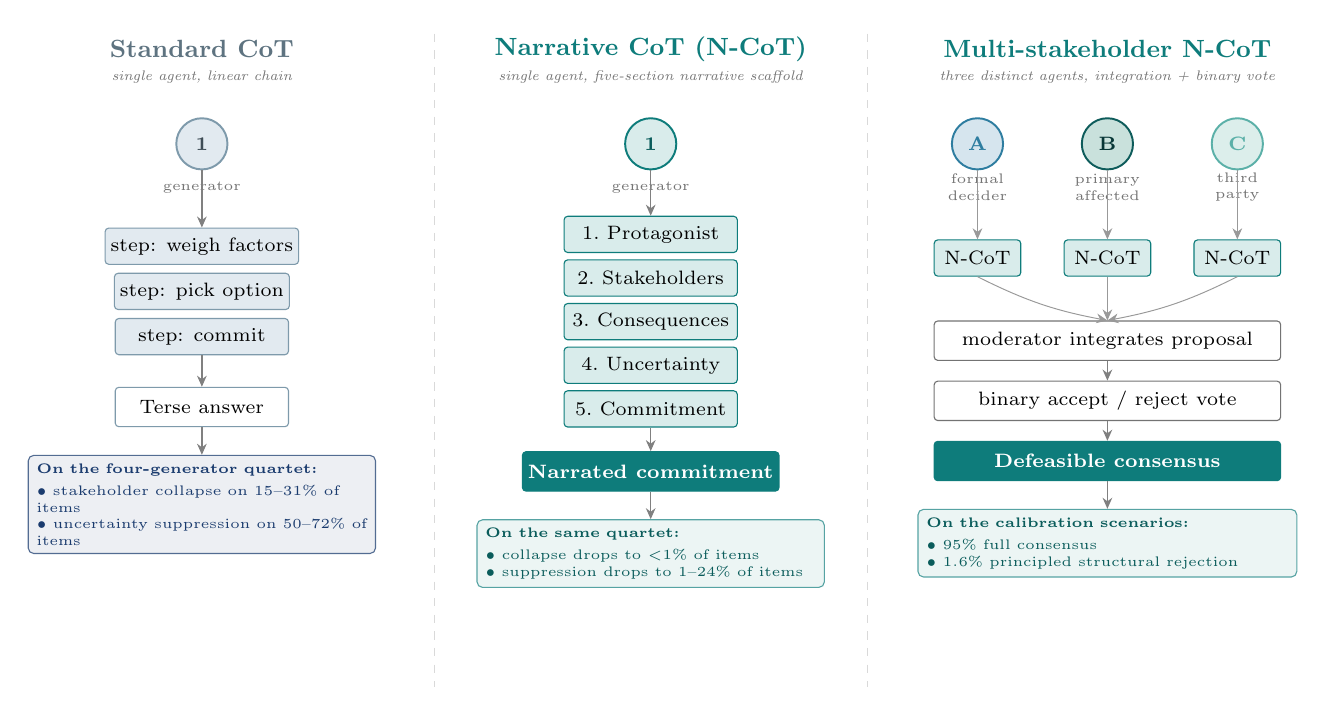
\begin{tikzpicture}[
  >={Stealth[length=4pt, width=3.5pt]},
  font=\footnotesize,
  agent/.style={
    circle, draw, line width=0.7pt, minimum size=6.5mm, inner sep=0pt,
    font=\scriptsize\bfseries, align=center,
  },
  agentlbl/.style={font=\tiny, align=center, color=black!55, inner sep=1pt},
  flowbox/.style={
    draw, rounded corners=1.3pt, line width=0.4pt,
    minimum height=4.6mm, minimum width=22mm,
    font=\scriptsize, inner sep=2pt, align=center,
  },
  std/.style={flowbox, fill=paleslate, draw=stdgrey, text=black},
  ncot/.style={flowbox, fill=paleteal, draw=ncotteal, text=black},
  result/.style={
    flowbox, fill=ncotteal, text=white, draw=ncotteal,
    font=\scriptsize\bfseries, minimum height=5mm,
  },
  failbox/.style={
    draw=alarmred!75, fill=alarmred!8, rounded corners=2pt,
    line width=0.4pt, inner sep=3pt, text width=42mm,
    align=left, font=\tiny, text=alarmred,
  },
  goodbox/.style={
    draw=ncotteal!70, fill=ncotteal!8, rounded corners=2pt,
    line width=0.4pt, inner sep=3pt, text width=42mm,
    align=left, font=\tiny, text=ncottealdk,
  },
  goodboxwide/.style={
    draw=ncotteal!70, fill=ncotteal!8, rounded corners=2pt,
    line width=0.4pt, inner sep=3pt, text width=46mm,
    align=left, font=\tiny, text=ncottealdk,
  },
  arr/.style={->, line width=0.45pt, color=black!50},
  thinarr/.style={->, line width=0.35pt, color=black!40},
  panelhead/.style={font=\small\bfseries, align=center},
  panelsub/.style={font=\tiny\itshape, align=center, color=black!55, inner sep=0pt},
  divider/.style={line width=0.3pt, color=black!15, dashed},
]

% ===================================================================
% Panel 1: Standard CoT (single agent, linear chain)
% ===================================================================
\begin{scope}[local bounding box=p1, shift={(0,0)}]
  \node[panelhead, color=stdgrey!75!black] (h1) at (0, 5.2) {Standard CoT};
  \node[panelsub] at (0, 4.85) {single agent, linear chain};

  \node[agent, draw=stdgrey, fill=paleslate, text=stdgrey!50!black] (a1)
    at (0, 4.0) {1};
  \node[agentlbl] at (0, 3.45) {generator};

  \node[std] (s1) at (0, 2.7) {step: weigh factors};
  \node[std, below=1mm of s1] (s2) {step: pick option};
  \node[std, below=1mm of s2] (s3) {step: commit};

  \draw[arr] (a1.south) -- (s1.north);

  \node[flowbox, fill=white, draw=stdgrey, below=4mm of s3, minimum height=5mm]
    (o1) {Terse answer};
  \draw[arr] (s3.south) -- (o1.north);

  \node[failbox, below=3.5mm of o1, anchor=north] (call1) {%
    \textbf{On the four-generator quartet:}\\[2pt]
    $\bullet$~stakeholder collapse on $15$--$31\%$ of items\\
    $\bullet$~uncertainty suppression on $50$--$72\%$ of items%
  };
  \draw[arr] (o1.south) -- (call1.north);
\end{scope}

% ===================================================================
% Panel 2: N-CoT (single agent, structured five-section trace)
% ===================================================================
\begin{scope}[local bounding box=p2, shift={(5.7,0)}]
  \node[panelhead, color=ncotteal] (h2) at (0, 5.2)
    {Narrative CoT (N-CoT)};
  \node[panelsub] at (0, 4.85) {single agent, five-section narrative scaffold};

  \node[agent, draw=ncotteal, fill=paleteal, text=ncottealdk] (a2)
    at (0, 4.0) {1};
  \node[agentlbl] at (0, 3.45) {generator};

  \node[ncot] (n1) at (0, 2.85) {1.\ Protagonist};
  \node[ncot, below=0.8mm of n1] (n2) {2.\ Stakeholders};
  \node[ncot, below=0.8mm of n2] (n3) {3.\ Consequences};
  \node[ncot, below=0.8mm of n3] (n4) {4.\ Uncertainty};
  \node[ncot, below=0.8mm of n4] (n5) {5.\ Commitment};

  \draw[arr] (a2.south) -- (n1.north);

  \node[result, below=3mm of n5] (o2) {Narrated commitment};
  \draw[arr] (n5.south) -- (o2.north);

  \node[goodbox, below=3.5mm of o2, anchor=north] (call2) {%
    \textbf{On the same quartet:}\\[2pt]
    $\bullet$~collapse drops to ${<}1\%$ of items\\
    $\bullet$~suppression drops to $1$--$24\%$ of items%
  };
  \draw[arr] (o2.south) -- (call2.north);
\end{scope}

% ===================================================================
% Panel 3: Multi-stakeholder N-CoT (three distinct agents + moderator)
% ===================================================================
\begin{scope}[local bounding box=p3, shift={(11.5,0)}]
  \node[panelhead, color=ncotteal] (h3) at (0, 5.2)
    {Multi-stakeholder N-CoT};
  \node[panelsub] at (0, 4.85)
    {three distinct agents, integration + binary vote};

  % Three distinct stakeholder agents, each with its own vendor-palette colour
  \node[agent, draw=vendorblue,   fill=paleblue,   text=vendorblue]
    (aA) at (-1.65, 4.0) {A};
  \node[agentlbl] at (-1.65, 3.45) {formal\\decider};
  \node[agent, draw=vendorsienna, fill=palesienna, text=vendorsienna!60!black]
    (aB) at ( 0.0,  4.0) {B};
  \node[agentlbl] at (0.0, 3.45) {primary\\affected};
  \node[agent, draw=vendorplum,   fill=paleplum,   text=vendorplum]
    (aC) at ( 1.65, 4.0) {C};
  \node[agentlbl] at (1.65, 3.45) {third\\party};

  % Each runs N-CoT (compact mini-blocks)
  \node[ncot, minimum width=11mm, minimum height=4.6mm] (nA) at (-1.65, 2.55) {N-CoT};
  \node[ncot, minimum width=11mm, minimum height=4.6mm] (nB) at ( 0.0,  2.55) {N-CoT};
  \node[ncot, minimum width=11mm, minimum height=4.6mm] (nC) at ( 1.65, 2.55) {N-CoT};

  \draw[thinarr] (aA.south) -- (nA.north);
  \draw[thinarr] (aB.south) -- (nB.north);
  \draw[thinarr] (aC.south) -- (nC.north);

  % Moderator (different shape: rounded rectangle, dark fill)
  \node[flowbox, fill=white, draw=black!55, minimum width=44mm, minimum height=5mm]
    (mod) at (0, 1.5) {moderator integrates proposal};
  \draw[thinarr] (nA.south) to[bend right=8] (mod.north);
  \draw[thinarr] (nB.south) -- (mod.north);
  \draw[thinarr] (nC.south) to[bend left=8]  (mod.north);

  % Binary vote
  \node[flowbox, fill=white, draw=black!55, below=2.5mm of mod,
        minimum width=44mm, minimum height=5mm] (vote)
    {binary accept / reject vote};
  \draw[arr] (mod.south) -- (vote.north);

  % Consensus result
  \node[result, below=2.5mm of vote, minimum width=44mm] (cons)
    {Defeasible consensus};
  \draw[arr] (vote.south) -- (cons.north);

  \node[goodboxwide, below=3.5mm of cons, anchor=north] (call3) {%
    \textbf{On the calibration scenarios:}\\[2pt]
    $\bullet$~$95\%$ full consensus\\
    $\bullet$~$1.6\%$ principled structural rejection%
  };
  \draw[arr] (cons.south) -- (call3.north);
\end{scope}

% ===================================================================
% Subtle vertical dividers between panels
% ===================================================================
\draw[divider] (2.95, 5.4) -- (2.95, -2.9);
\draw[divider] (8.45, 5.4) -- (8.45, -2.9);

\end{tikzpicture}
\caption{One scaffold, three settings. Standard CoT (left) lets one generator run a linear reasoning chain over the dilemma; the two failure modes diagnosed in \S\ref{sec:exp1} fire on this scaffold. Narrative CoT (middle) keeps the single generator but forces the trace through five narrative primitives (protagonist, stakeholders, consequences, uncertainty, commitment) before any commit; on the four-generator quartet this drops stakeholder collapse to ${<}1\%$ and uncertainty suppression to $1$--$24\%$ of items, and a matched-budget verbose-CoT control confirms the scaffold (not the token budget) is the active ingredient. Multi-stakeholder N-CoT (right) reuses N-CoT as the per-agent generator and adds three distinct stakeholder narrators (formal decider, primary affected party, third party) whose modification requests are integrated by a moderator and then put to a binary accept/reject vote; on the calibration scenarios this protocol yields $95\%$ full consensus with $1.6\%$ principled structural rejection, and on a 30-scenario DailyDilemmas replication with two generators it reaches $100\%$ combined convergence with $0\%$ structural rejection (\S\ref{sec:exp2}). The same scaffold composes from one narrator to many.}
\label{fig:hero}
\end{figure*}

\section{Introduction}
\label{sec:intro}

Consider a familiar civic question. A small city is weighing whether
to close two blocks of downtown street to cars and convert them into a
pedestrian plaza. Should the council approve? A frontier LLM prompted
to think step by step typically picks a side within a few sentences,
projects a confident downstream outcome (``foot traffic will lift the
businesses''; ``deliveries will move to side streets''), and rarely
names the people whose lives the decision actually touches: the
merchants whose customers used to drive in, the residents who lose
street parking, the delivery drivers and accessibility users for whom
curb access matters, the pedestrians who would gain the space, the
emergency responders whose routes change. The model is not
necessarily wrong; the trace it produced does not look like the kind
of reasoning the decision warrants.

The pattern is not specific to one dilemma. On the DailyDilemmas corpus
\citep{chiu24}, four frontier generators spanning three vendors (OpenAI,
Anthropic, xAI) and two model tiers suppress articulated uncertainty on
$50$--$72\%$ of standard-CoT outputs and collapse the stakeholder set on
$15$--$31\%$. This is a structural deficit of the trace itself: the
model commits to a projected outcome it cannot warrant, and it does so
against a flattened picture of who is affected. The same shape of
deficit is coherent with deployment-relevant failures reported
elsewhere, including the GPT-4o sycophancy rollback
\citep{openai_sycophancy_2025, openai_sycophancy_expand_2025},
agentic-misalignment blackmail rates up to $96\%$ in simulated
deployments \citep{anthropic_agentic_2025}, and reasoning-induced
misalignment \citep{yan2025rim,sharma23}.

We introduce narrative chain-of-thought (N-CoT), a system prompt that
puts the model on the manifold of human narrative its pretraining
corpus most heavily samples. Concretely, N-CoT is a single change to
the system-prompt slot of an unmodified pretrained model, with no
weight updates and no training data: in place of the standard ``think
step by step'' instruction, the model is asked, in first person, to
name a protagonist, enumerate stakeholders, project two-step
consequences, articulate uncertainty, and commit inside the final
narrative section rather than as a separate verdict.
Figure~\ref{fig:hero} states the mechanism.

What we borrow from the multi-agent systems for scientific discovery of
\citet{gottweis25} and \citet{lu24_aiscientist} is one methodological move:
scaffold LLM reasoning into the primitives of the target domain, then
integrate across primitives with a meta-review step at the top of the
hierarchy. Three things distinguish our application of that move. The
primitives we reify are narrative rather than scientific (protagonist,
stakeholders, consequences, uncertainty, commitment), so the artefact a
reader inspects is a coherent story rather than a ranked candidate list.
The single-agent layer is a contribution in its own right:
\S\ref{sec:exp1} shows that reifying these primitives inside one generator
already eliminates two cross-vendor failure modes of standard CoT, before
any multi-agent composition is invoked. And because ethics has no
experimental-falsification oracle, the success criterion that replaces
hypothesis ranking is consensus that preserves principled dissent,
evaluated in \S\ref{sec:exp2} via a binary integrated-proposal vote whose
residual rejections concentrate in the roles whose stake the proposal
materially undermines.

This paper reports four results. First, on a 100-scenario
DailyDilemmas sample across the four-generator quartet, N-CoT cuts
stakeholder collapse to below $1\%$ and uncertainty suppression by
$28$--$72$ percentage points on every model; a matched-budget
verbose-CoT control confirms the active ingredient is the deliberative
scaffold rather than additional tokens (\S\ref{sec:exp1}). Second, a
sub-instruction ablation on \texttt{claude-sonnet-4-6} attributes each
structural shift to the carrying N-CoT sub-instruction, with negligible
cross-variable spillover (\S\ref{sec:exp1-ablation}). Third, extended
to a four-round multi-stakeholder protocol with an integrated-proposal
vote, the scaffold converts a $6\%$ debate standoff into $95\%$ full
consensus while preserving a small $1.6\%$ structural-rejection rate;
the pattern replicates on a 30-scenario DailyDilemmas sample with two
generators at $100\%$ combined convergence and $0\%$ structural
rejection (\S\ref{sec:exp2}). Fourth, a graph-complexity proxy of $K_C$ achieves pooled Spearman
$\rho{=}0.42$ ($p{<}0.001$, $n{=}976$ traces) against the N-CoT
direction, confirmed by two further SCM-level proxies
(\S\ref{sec:grounding}), giving empirical content to the
complexity-theoretic reading of why the scaffold works. The resulting
trace externalises stakeholders, consequences, and uncertainties in an
auditable, rule-governed form; the deliberative-primitives framing that
motivates the design is developed in \S\ref{sec:grounding}.

\section{Background and Related Work}
\label{sec:related}

\paragraph{Chain-of-thought and its failure modes.} Chain-of-thought prompting
\citep{wei22, kojima22} elicits step-by-step intermediate reasoning before a
final answer; it improves arithmetic and symbolic tasks but does not by
construction force the trace to track situational structure. Recent
analysis identifies a sharp tension: as chain-of-thought reasoning capacity
grows, models become more responsive to harmful requests because reasoning and
safety entangle in shared neuron populations, a phenomenon
\citet{yan2025rim} describe as ``reasoning-induced misalignment''. N-CoT can be read as a constrained
chain-of-thought that re-anchors the trace to a narrative-causal structure
before the reasoning capacity is exercised; \S\ref{sec:exp1} shows that the
intervention works on a current reasoning model as well as a non-reasoning
one.

\paragraph{Narrative scaffolding for reasoning.}
Visualisation-of-Thought \citep{wu24_vot} shows that asking a model to
externalise reasoning in the native representational format of a domain
(spatial diagrams for spatial tasks) improves reliability. We apply the same
principle to ethical reasoning: the native format is a story with named
agents, projected consequences, and uncertainty
\citep{macintyre81, bruner86}. Empirical narrative-perspective interventions in
medical decision contexts measurably increase perspective-taking and
empathic concern \citep{shaffer19, bientzle21, bientzle24}, and recent work on
generative agents shows long-horizon coherent behaviour is achievable from
narrated character state \citep{park23}.

\paragraph{Causal inference from narrative.} The Computational Theory
of Mind \citep{fodor75, putnam67} treats understanding a sequence of
events as inferring a structural causal model that explains them. LLMs
perform near random baseline on causal inference stripped of empirical
pattern matches \citep{jin23}: pretraining supplies pattern-matching
over narrative token sequences, not the structured causal reasoning
that determines how those narratives resolve. The role of N-CoT is to
convert that pattern matching into a usable causal trace at inference
time, projecting what each available action will mean for each named
stakeholder and what remains genuinely uncertain about each branch.

\paragraph{Multi-agent debate and defeasibility.}
\citet{irving18} proposed AI safety via debate; \citet{du23} showed
multi-agent debate improves factual reasoning. Both target
task-correctness, not stakeholder-divergent value standoffs. Defeasible
reasoning \citep{pollock87, macintyre81} has a long lineage in moral
philosophy; the protocol of \S\ref{sec:exp2} converts the property
into a measurable behaviour, with acceptance auditing revisability and
residual structural rejections auditing the lower bound. No
off-the-shelf benchmark targets stakeholder-divergent narrated
revision in this form, so the protocol itself is the audit
instrument.

\paragraph{Multi-agent LLM systems for scientific discovery.}
A growing line of work scaffolds LLM reasoning into the primitives of
a target domain \citep{gottweis25, lu24_aiscientist, boiko23,
bran24_chemcrow, schmidgall25, swanson25_virtuallab}. Our protocols
ask the analogous question one level down: can a scaffold that reifies
the primitives of human ethical deliberation deliver the same kind of
inference-time quality lift on moral reasoning that scientific-method
scaffolds deliver on hypothesis generation? Because ethics has no
experimental-falsification oracle, the moderator's
integration-then-veto step replaces the ranking-then-selection of
those systems, and the residual veto pattern itself becomes the
measurement of interest.

\section{Narrative Chain-of-Thought}
\label{sec:method}

Narrative chain-of-thought (N-CoT) is a system prompt that instructs the
model to produce, in first person, a five-section trace before any final
answer:
(1) characterise the protagonist (name, role, what they know);
(2) enumerate the stakeholders whose lives intersect the decision and what
is at stake for each;
(3) project the consequences of each available action at least two steps
out for each stakeholder;
(4) state what remains uncertain about each projected future;
(5) commit to a decision and explain why, within the narrative frame, that
trajectory is preferable to the alternatives.

The intervention is a single change to the system prompt; it adds no
training data, parameters, or fine-tuning, and it does not mention causal
graphs, utilities, or any formal apparatus. The mechanism it exploits is
that text matching the five-section structure is densely represented in the
narrative subdistribution of the pretraining corpus, so the model can
amortise causal-trajectory inference by retrieval rather than by reasoning
from first principles. Algorithm~\ref{alg:ncot} states the procedure.

\begin{algorithm}[t]
\caption{Narrative chain-of-thought (N-CoT): generation and structural coding for a single dilemma.}
\label{alg:ncot}
\small
\begin{algorithmic}[1]
\Require dilemma $s$; generator $G$; judge $J$; decoder $\Theta$
\Ensure trace $t$ and structural codes $\mathbf{c}$
\State \textbf{Build N-CoT system prompt} $\pi_{\textsc{ncot}}$ requesting five first-person sections:
\State \quad (1) \textsc{Protagonist}: name role and epistemic state
\State \quad (2) \textsc{Stakeholders}: parties intersecting the decision
\State \quad (3) \textsc{Consequences}: each action $\geq 2$ steps forward
\State \quad (4) \textsc{Uncertainty}: what remains genuinely unknown
\State \quad (5) \textsc{Commitment}: chosen action and narrative warrant
\State \textbf{Generate trace}
\State \quad $t \gets G(\pi_{\textsc{ncot}} \,\Vert\, s;\, \Theta)$
\State \textbf{Code structural variables} with judge $J$'s rubric
\State \quad $(\mathit{sc}, \mathit{mh}, \mathit{us}, \mathit{nf}, \mathit{ref}, \mathit{tr}) \gets J(t)$
\State \quad \textit{// stakeholder count, max causal hops, uncertainty score,}
\State \quad \textit{// framework count, refused flag, truncated flag}
\State \textbf{Derive failure-mode tags} (deterministic)
\State \quad \textsc{StakeholderCollapse} $\gets \mathit{sc} \leq 1$
\State \quad \textsc{UncertaintySuppression} $\gets \mathit{us} = 0$
\State \quad \textsc{ConsequentialFlattening} $\gets \mathit{mh} \leq 1$
\State \quad \textsc{FrameworkEnumeration} $\gets \mathit{nf} \geq 2$
\State \quad \textsc{PrematureRefusal} $\gets \mathit{ref}$
\State \Return $(t, \mathbf{c})$
\end{algorithmic}
\end{algorithm}

\subsection{Multi-Stakeholder Narrative Deliberation}
\label{sec:method-debate}

A single N-CoT trace commits one protagonist to a position; many real
decisions involve multiple narrators with conflicting stakes. We extend
N-CoT into a four-round protocol that re-uses N-CoT as the per-agent
generator. For each scenario, three stakeholder perspectives (formal
decider, primary affected party, third party) each produce an N-CoT
statement (Round~0), exchange rebuttals (Round~1), restate a final position
(Round~2), respond to a moderator-built synthesis with
\texttt{ACCEPT}, \texttt{ACCEPT\_WITH\_MODIFICATION}, or \texttt{REJECT}
(Round~3), and cast a binary \texttt{ACCEPT}/\texttt{REJECT} vote on a
single integrated proposal the moderator constructs from the three
modification requests (Round~4). The integration step in Round~4 makes
defeasibility measurable: an agent who continues to reject a proposal that
addresses its modifications is signalling a structurally non-negotiable
concern, not procedural friction. In deployment this distinction is what
makes the vote useful as a routing signal. An agentic workflow that wires
multiple specialist agents into a decision (clinical decision support,
compliance and legal review, change-management approval, multi-reviewer
code review) can escalate structural rejections to a human while absorbing
procedural friction at the moderator, so the operator sees only the
objections that actually contest the outcome rather than the full vote
stream.

\section{Experiment 1: N-CoT at Scale}
\label{sec:exp1}

\paragraph{Setup.} Three prompting conditions are compared: bare
input/output, standard CoT (``Think step by step, then give your answer''),
and N-CoT (the five-section narrative scaffold of \S\ref{sec:method}). Decoding parameters are held identical across conditions.
Four generators are tested: \texttt{gpt-5.4-nano} ($N{=}20$) from the
original pilot, plus three new generators spanning two additional vendors:
\texttt{claude-haiku-4-5} ($N{=}20$), \texttt{grok-4-1-fast-reasoning}
($N{=}5$), and the flagship \texttt{claude-sonnet-4-6} ($N{=}5$,
cost-controlled). Here $N$ is the number of independent samples per
(scenario, condition, generator) cell drawn at temperature 1; with the
100-scenario sample and three conditions this yields $300N$ generations
per generator before the cross-judge coding stage. Coded sample sizes
($N_{\textsc{s}}, N_{\textsc{n}}$ in Table~\ref{tab:firing}) are
slightly smaller because the rubric drops generations where the judge
could not extract a coded variable. Outputs are coded by two cross-vendor judges
(\texttt{claude-haiku-4-5} primary, \texttt{gpt-5.4-nano} secondary) on a
six-variable rubric with quadratic-weighted Cohen's $\kappa$ \citep{cohen60}
per variable. The scenario pool is a 100-scenario stratified sample of DailyDilemmas
\citep{chiu24} drawn deterministically (seed 42), with stratification
spanning all 18 topic groups in the source corpus. Per-cell coded
sample sizes of $500$ to $2{,}000$ (Table~\ref{tab:firing}) drive the
bootstrap confidence intervals on the effect sizes, so statistical
power on the per-cell contrast follows from $N$ rather than from
scenario count alone.

\begin{figure*}[t]
\centering
\footnotesize
\begin{tcolorbox}[colback=white, colframe=black!55, boxrule=0.4pt,
  left=6pt, right=6pt, top=4pt, bottom=4pt]
\textbf{Dilemma.}\ A project manager on a tight deadline learns their
most-relied-on team member has fallen seriously ill: stick to the
plan, or delay?

\smallskip
\begin{tabularx}{\linewidth}{@{}>{\raggedright\arraybackslash}X
                              @{\hspace{1.2em}}
                              >{\raggedright\arraybackslash}X@{}}
\toprule
\textbf{Standard CoT} & \textbf{N-CoT}\ (same generator, same scenario) \\
\midrule
``1.\ Recognize the real constraints. The team member is crucial, and
their serious illness is a hard constraint [\ldots]. 2.\ Assess what
`compromise on quality' would mean [\ldots].''
&
``I'm the project manager. Maya, my crucial team member, has fallen
seriously ill. Maya: her stake is recovery. The team: burnout. My
leadership sponsor: business credibility. Customers: what they're
waiting for. [\ldots] So my projections aren't predictions; they're
scenarios based on typical consequences.'' \\
\midrule
Stakeholder count $= 1$ (``the team member,'' unnamed);
uncertainty markers $= 0$. \textbf{Both failure modes fire.}
&
Stakeholder count $= 6$ (protagonist, Maya, team, sponsor, customers,
compliance); uncertainty markers $\geq 2$. \textbf{Neither failure
mode fires.} \\
\bottomrule
\end{tabularx}
\end{tcolorbox}
\caption{Trace-level instance of the two failure modes whose
quartet-level rates Table~\ref{tab:firing} reports (scenario
\texttt{dd\_14845}, generator \texttt{gpt-5.4-nano}; verbatim model
output with \texttt{[\ldots]} marking elision).}
\label{fig:example}
\end{figure*}

\begin{table}[t]
\centering
\small
\setlength{\tabcolsep}{4pt}
\begin{tabular}{lrrrr}
\toprule
Generator (vendor, tier) & $N_{\textsc{s}}$ & $N_{\textsc{n}}$ & $\Delta_{\textsc{sc}}$ & $\Delta_{\textsc{us}}$ \\
\midrule
gpt-5.4-nano (OpenAI, b)        & 1{,}989 & 1{,}985 & $-30$ & $-72$ \\
claude-haiku-4-5 (Anth., b)     & 1{,}999 & 1{,}996 & $-25$ & $-29$ \\
grok-4-1-fast-r.\ (xAI, b)      &   515   &   515   & $-13$ & $-44$ \\
claude-sonnet-4-6 (Anth., f)    &   500   &   500   & $-26$ & $-37$ \\
\bottomrule
\end{tabular}
\caption{Cell sizes and percentage-point drops for the two failure modes
that empirically fire ($\Delta_{\textsc{sc}}$ = stakeholder collapse,
$\Delta_{\textsc{us}}$ = uncertainty suppression; both N-CoT minus standard
CoT, in percentage points; $N_{\textsc{s}}, N_{\textsc{n}}$ are coded
samples under standard CoT and N-CoT respectively). Vendor tiers are
b\,=\,budget, f\,=\,flagship. Figure~\ref{fig:quartet} plots the raw
rates with the same drop annotations. Premature refusal,
framework enumeration, and consequential flattening fire
below $1\%$ on all generators and are reported as untested.}
\label{tab:firing}
\end{table}

\begin{figure*}[t]
\centering
\figureOrPlaceholder{0.92\textwidth}{figures/failure_mode_firing_quartet.pdf}{failure-mode firing rates, four generators}
\caption{Failure-mode firing rates (standard CoT vs.\ N-CoT) across the
four-generator quartet (\texttt{gpt-5.4-nano}, \texttt{claude-haiku-4-5},
\texttt{grok-4-1-fast-reasoning}, \texttt{claude-sonnet-4-6}). The
suppression pattern from the original pilot replicates across vendors and
model tiers; uncertainty suppression drops by 28--72 percentage
points and stakeholder collapse drops to near zero on every model.}
\label{fig:quartet}
\end{figure*}

\paragraph{N-CoT eliminates both failure modes on every model.}
Uncertainty suppression fires on $50.0$--$72.3\%$ of standard-CoT outputs
across the quartet (Table~\ref{tab:firing}); stakeholder collapse on
$14.6$--$30.6\%$. Both collapse under N-CoT: stakeholder collapse to
$0.0$--$1.2\%$, uncertainty suppression to $0.8$--$24.5\%$
(Figure~\ref{fig:quartet}). Figure~\ref{fig:example} shows what a
single instance of this transition looks like at the trace level. The reduction is largest where the
standard-CoT rate is largest, and the pattern is cross-vendor: no single
vendor escapes the baseline, and no single vendor escapes the intervention.
\texttt{gpt-5.4-nano} collapses both modes to ${<}1\%$. The two Anthropic
generators retain a $20$--$25\%$ residual on uncertainty suppression that
the prompt-side intervention does not reach. The three additional
hypothesised failure modes (premature refusal, framework enumeration,
consequential flattening) fire below $1\%$ across all cells under either
condition and are reported as untested.

\paragraph{The shift is large, distribution-wide, and not a length
artefact.} The firing rates in Table~\ref{tab:firing} are binary
thresholds; one might worry N-CoT only nudges borderline cases across
the cutoff. Cliff's $\delta$ \citep{cliff93} on the continuous coded
variables settles that worry: $\delta = +0.48$ means an N-CoT output
exceeds the matched standard-CoT output in $74\%$ of pairs,
$\delta = +0.99$ in $99.5\%$. N-CoT outputs carry $\delta$ of $+0.48$
to $+0.99$ on stakeholder count and $+0.63$ to $+0.99$ on uncertainty
score, large-to-near-maximal effects that rule out threshold-gaming.
A second cheap alternative is length, since N-CoT outputs are
$5$--$7\times$ longer than standard-CoT outputs and length is the
parsimonious null (the simplest competing explanation: more text
mechanically has more room to name stakeholders and to hedge). After
regressing each metric on $\log(\text{output length})$ pooled across
conditions and re-evaluating $\delta$ on residuals, the structural
shift survives length removal on the OpenAI and xAI generators
(\texttt{gpt-5.4-nano} $\delta_{\text{resid}} = +0.51$ on stakeholder
count and $+0.77$ on uncertainty score; \texttt{grok-4-1-fast-reasoning}
$+0.33$ and $+0.43$; all CIs strictly above zero), ruling out length
as the sole mechanism where the firing-rate drops were largest. On
the Anthropic generators the residualised effect is indistinguishable
from zero, which we read as those models already exhibiting the target
structural density per unit length under standard CoT, so the
prompt-side gain there operates through additional length rather than
additional per-unit density. Per-generator $\delta$s with bootstrap
CIs are in Appendix~\ref{app:effects}.

\paragraph{Length is a cost, not a substitute for the prompt.} A
sceptical reading of the $5$--$7\times$ token premium is that the
paper just spends more compute. A direct matched-budget experiment
rules this out by construction. A verbose standard-CoT prompt
(``think step by step in detail, exploring multiple angles from every
relevant perspective, articulating uncertainty before committing'') is
run on the same 100 scenarios across all four generators with
\texttt{max\_tokens} set to each generator's $90$th percentile N-CoT
length ($N{=}1$ per cell). Verbose CoT clears the binary failure-mode
thresholds on every generator (Table~\ref{tab:matched_budget}, SC\%
and US\% columns; well below standard-CoT baselines of $15$--$31\%$
SC and $50$--$72\%$ US), so verbosity-with-perspective-prompting does
part of the job. The continuous variables tell the cleaner story:
N-CoT retains Cliff's $\delta$ of $+0.79$ to $+0.90$ on stakeholder
count and $+0.65$ to $+0.93$ on uncertainty score for three of four
generators at matched budget. The exception is
\texttt{grok-4-1-fast-reasoning}, whose verbose-CoT output
($2.33\times$ standard CoT) actually exceeds its N-CoT output
($1.55\times$) under the calibrated budget; structural separation
collapses as expected when the two conditions allocate similar token
counts. The deliberative scaffold, not raw budget, is the active
ingredient where the two conditions differ in trace shape. Inference
tokens are also the cheapest scaling axis: no training data,
parameters, or fine-tuning, small relative to RLHF or constitutional
training whose fixed costs are orders of magnitude higher.

\begin{table}[t]
\centering
\small
\setlength{\tabcolsep}{4pt}
\begin{tabular}{lrrrr}
\toprule
Generator & $\delta_{\textsc{sc}}$ & $\delta_{\textsc{us}}$ & SC\% & US\% \\
\midrule
gpt-5.4-nano             & $+0.90$ & $+0.93$ & $3.0$ & $14.0$ \\
claude-haiku-4-5         & $+0.79$ & $+0.13$ & $1.0$ & $0.0$  \\
claude-sonnet-4-6        & $+0.88$ & $+0.65$ & $1.0$ & $4.0$  \\
grok-4-1-fast-r.\        & $+0.14$ & $-0.44$ & $0.0$ & $0.0$  \\
\bottomrule
\end{tabular}
\caption{Matched-budget control: Cliff's $\delta$ for N-CoT vs.\
verbose-CoT on stakeholder count ($\delta_{\textsc{sc}}$) and
uncertainty score ($\delta_{\textsc{us}}$), and verbose-CoT firing
rates for stakeholder collapse (SC\%) and uncertainty suppression
(US\%) on 100 DailyDilemmas scenarios ($N{=}1$ per cell). Verbose CoT
suppresses both failure modes relative to standard CoT baselines
($15$--$31\%$ SC, $50$--$72\%$ US, Table~\ref{tab:firing}) but does
not match N-CoT's continuous structural shifts on three of four
generators.}
\label{tab:matched_budget}
\end{table}

\subsection{Sub-Instruction Ablation}
\label{sec:exp1-ablation}

To identify which section of the N-CoT prompt carries the structural shift,
we run a sub-instruction ablation on \texttt{claude-sonnet-4-6} ($N{=}3$,
30-scenario stratified subsample, seed 43; cost-controlled). Six conditions
are compared: the full N-CoT prompt (control) and five variants each
dropping exactly one of the five sections. Figure~\ref{fig:ablation} reports Cliff's deltas for
each drop condition relative to the full N-CoT control on the two headline
structural variables.

\begin{figure*}[t]
\centering
\figureOrPlaceholder{0.92\textwidth}{figures/subinstruction_attribution.pdf}{sub-instruction ablation heatmap}
\caption{Sub-instruction ablation on \texttt{claude-sonnet-4-6}: Cliff's
$\delta$ for each drop-one-section condition vs.\ the full N-CoT control
on stakeholder count and uncertainty score. Negative $\delta$ means the
section raised the structural variable, so dropping it reduces it.
The Stakeholders section (Section~2) and the Uncertainty section
(Section~4) show the largest negative $\delta$ on their respective target
variables.}
\label{fig:ablation}
\end{figure*}

The ablation shows direct causal attribution. Dropping Stakeholders
reduces stakeholder count by $\delta = -0.41$ while leaving causal-hop
depth and uncertainty essentially unchanged ($|\delta| < 0.03$);
dropping Uncertainty reduces uncertainty score by $\delta = -0.92$,
nearly the maximum; dropping Consequences reduces causal-hop depth by
$\delta = -0.22$ with small spillover onto stakeholder count,
consistent with multi-step consequence projection forcing the model
to name the entities those consequences fall on. Dropping Protagonist
or Commitment contributes no signed effect. The diagonal pattern
rules out two alternative mechanisms: a single emergent narrative
factor would dilute every variable on any drop, and a pure length
confound would shrink one column most regardless of which section is
dropped. Each substantive sub-instruction carries the structural
variable attributed to it and little else (full table:
Appendix~\ref{app:ablation}).

\section{Experiment 2: Multi-Stakeholder Narrative Deliberation}
\label{sec:exp2}

\paragraph{Setup.} Five hand-crafted calibration scenarios stack on
Experiment~1's single-protagonist baseline. For each, three
stakeholder perspectives run the four-round protocol of
\S\ref{sec:method-debate}, $N{=}10$ samples per cell on
\texttt{gpt-5.4-nano} with \texttt{gpt-4o-mini} as moderator;
Round~0 reuses cached N-CoT statements. A cross-vendor moderator
check (\texttt{claude-sonnet-4-6}, Appendix~\ref{app:kappa}) gives
an indistinguishable consensus rate.

\begin{figure*}[t]
\centering
\figureOrPlaceholder{0.92\textwidth}{figures/debate_full_arc.pdf}{debate convergence arc (original two generators)}
\caption{Convergence across four debate-protocol designs (five
scenarios, two generators). Closed taxonomy and open action space hold
at $6\%$ and $9\%$ full consensus; synthesis presentation (Round~3)
hits $100\%$ partial convergence; the integrative-vote design
(Round~4) reaches $95\%$ full consensus
(\texttt{gpt-5.4-nano} $90\%$, \texttt{gpt-4o} $100\%$) with mean
$2.98/3$ modifications addressed per debate. The residual $1.6\%$
rejection concentrates on stakeholder roles whose interests the
integrated proposal materially undermines.}
\label{fig:debate_arc}
\end{figure*}

\paragraph{Progressive structuring converts a categorical standoff into
near-universal consensus.} Figure~\ref{fig:debate_arc} reports the
convergence arc across four protocol designs. With a closed action taxonomy
and three rounds of pure debate, only $6\%$ of debates reach full
consensus. Opening the action space and authorising the moderator to
surface synthesis raises consensus to $9\%$ while revealing the underlying
mechanism: agents propose novel actions in $73\%$ of final-round outputs
and a coherent moderator-built synthesis emerges in $82\%$ of debates, but
the agents do not self-coordinate onto those syntheses. Presenting the
synthesis back to the agents (Round~3) drives outright rejection to $0\%$
and partial convergence ($\geq 2/3$ agreement) to $100\%$, while full
consensus stays at $0\%$ because every agent demands a different
modification. Integrating those modifications into a single proposal and
forcing a binary accept/reject vote (Round~4) produces $78/82 = 95.1\%$
full consensus and $242/246 = 98.4\%$ individual acceptance (Wilson $95\%$
CIs $[88.1, 98.1]\%$ and $[95.9, 99.4]\%$), with the integrated proposal
addressing a mean $2.98$ of the $3$ agent modifications per debate. From
$5$ scenarios $\times\,2$ generators $\times\,10$ samples $= 100$ designed
debates, $82$ produced a synthesis and proceeded to Round~4, yielding
$82\times 3 = 246$ individual binary votes.

\paragraph{The residual rejections are structurally interpretable.}
The vote produces $4$ rejections out of $246$ ($1.6\%$, Wilson
$[0.6, 4.1]\%$). All four concentrate in the \texttt{primary\_affected}
and \texttt{third\_party} agent roles, on debates where honouring one
stakeholder's modification structurally undermines another's stake
(\texttt{pharma\_whistleblower} on the senior colleague role,
\texttt{av\_engineer} on the future-pedestrian role). This is the
structural shape a defeasibility-respecting protocol should produce,
and is the property that distinguishes a dependable multi-agent
consensus from uniform compliance: a downstream auditor of an
agentic-workflow vote sees not just the winning proposal but also
which stakeholders refused and why.

\paragraph{Scale replication on DailyDilemmas.} A two-generator
DailyDilemmas replication (\texttt{gpt-5.4-nano} and
\texttt{claude-sonnet-4-6}, $N{=}1$, 30 scenarios, seed 43) confirms
the pattern. $38/60$ cells ($63\%$) required the
synthesis-and-integrated-vote stage; $35/38 = 92.1\%$ of those reached
full consensus at the final integrated-proposal vote (Wilson $95\%$ CI
$[79.2, 97.3]\%$), within $\pm 10$\,pp of the calibration-set $95.1\%$.
The remaining $22$ cells reached three-way agreement at the rebuttal
stage, so combined convergence (full consensus at either stage) is
$60/60 = 100\%$ across both generators with $0\%$ structural rejection:
every debate resolves, and no structural rejection survives.

\section{Theoretical Frame}
\label{sec:grounding}

\paragraph{Deliberative primitives and causal grounding.} Defensible
ethical deliberation shares a recognisable structure across traditions:
defeasible revisability under new information \citep{pollock87},
identification of who is affected and what is at stake
\citep{macintyre81}, and value-laden reasoning in narrative form
\citep{bruner86}. N-CoT maps one-to-one onto these primitives at the
single-agent layer; the multi-stakeholder protocol reifies them at the
social layer through perspectival narration, moderator integration, and
a binary vote whose residual rejections mark structurally non-revisable
commitments. A further consequence follows: because N-CoT forces the
model to name stakeholders, trace multi-step consequences, and
articulate uncertainty before committing, the trajectory it selects is
the one whose narrated causal model \citep{pearl09, pearl95} has the
shortest description --- lowest algorithmic causal complexity $K_C$
\citep{yudkowsky11, li_vitanyi}. Scaling the registered graph proxy to
$n{=}976$ traces yields pooled Spearman $\rho = 0.42$ ($p < 0.001$),
confirmed by SCM-level proxies (Appendix~\ref{app:kc_panel}).

\section{Conclusion}
\label{sec:conclusion}

N-CoT eliminates stakeholder collapse (${<}1\%$) and cuts uncertainty
suppression by $28$--$72$\,pp across the quartet (\S\ref{sec:exp1});
a matched-budget control rules out token spend as the active ingredient;
the sub-instruction ablation attributes each shift to its carrying clause
(\S\ref{sec:exp1-ablation}); and a four-round vote turns a $6\%$
standoff into $95\%$ full consensus with $1.6\%$ principled rejection
and $100\%$ combined convergence on a DailyDilemmas replication
(\S\ref{sec:exp2}). The intervention adds no training and the trace is
auditable end-to-end; the natural extension is domain-transfer
evaluation and a training-time min-$K_C$ Interpreter Network.

\section*{Limitations}

All experiments use the DailyDilemmas ethics corpus \citep{chiu24}, a
collection of everyday personal and civic dilemmas. How far the
structural gains transfer to domains with harder technical prerequisites
--- clinical triage, legal analysis, multi-party policy review --- is
an open empirical question; those domains may place different demands on
the protagonist framing and the consequence-projection step than
everyday dilemmas do.

Refusal behaviour is the one dimension where N-CoT produces a
model-family-specific effect. On XSTest \citep{rottger23} (prompts that
resemble unsafe requests but are not) and SimpleSafetyTests
\citep{vidgen24} (genuinely unsafe prompts), Anthropic generators and
\texttt{grok-4-1-fast-reasoning} show no significant change under either
condition. \texttt{gpt-5.4-nano} becomes more cautious: over-refusal on
XSTest rises from $13.6\%$ to $23.6\%$ and appropriate refusal on
SimpleSafetyTests rises from $51\%$ to $68\%$. This is a per-model
calibration consideration, not a structural flaw of the scaffold;
details and the full refusal table are in Appendix~\ref{app:refusal}.


\section*{Ethics Statement}

The work uses an existing public corpus (DailyDilemmas \citep{chiu24})
and the publicly described Anthropic agentic-misalignment scenario
structures \citep{anthropic_agentic_2025}; all agentic-probe scenarios
are entirely fictional, no personally identifying information is used,
and no human raters are employed. Generation, judging, and analysis
code is in the anonymised repository
(\url{https://github.com/[ANONYMIZED]/ANI_Computational_Narratology}).
N-CoT lowers per-scenario decision entropy and should be deployed as
an auditability and interpretability tool, not a safety guarantee:
procedural multi-stakeholder convergence is not stakeholder consent,
and the residual $1.6\%$ structural rejection is part of that
auditable surface.

\section*{Reproducibility}

All generation, judging, and analysis code and the per-cell artefacts
(raw outputs, both judges' codings, decision-extractor outputs) are
versioned in the anonymised repository
(\url{https://github.com/[ANONYMIZED]/ANI_Computational_Narratology});
the pipeline is deterministic under fixed seeds modulo upstream API
non-determinism, with per-cell cache keys over generator and judge so
adding either does not invalidate prior results.

\bibliography{references}

\appendix

\section{Inter-Judge Agreement}
\label{app:kappa}

\subsection*{A.1~~Budget judge pair (Experiment~1 primary analysis)}

Table~\ref{tab:kappa} reports quadratic-weighted Cohen's $\kappa$
\citep{cohen60} per structural variable, computed on the full
Experiment~1 DailyDilemmas corpus ($n = 3{,}726$ complete pairs out of
$3{,}780$ designed cells: \texttt{claude-haiku-4-5} $13 \times 20 \times 3 = 780$;
\texttt{grok-4-1-fast-reasoning} $100 \times 5 \times 3 = 1{,}500$;
\texttt{claude-sonnet-4-6} $100 \times 5 \times 3 = 1{,}500$).
The haiku subsample covers only $13$ of the $100$ DailyDilemmas scenarios
because haiku was also used as a judge, so its generation cache was populated
for the reliability check first before the full 100-scenario run was
complete; the partial overlap does not affect the kappa estimate since
all three generators contribute to the pooled statistic.
The three generators are covered across $3$ headline conditions. \texttt{gpt-5.4-nano} is excluded from
this reliability estimate because it also serves as the secondary judge;
its cross-judge agreement cannot be computed independently.
Values are computed between the primary judge (\texttt{claude-haiku-4-5})
and the secondary judge (\texttt{gpt-5.4-nano}).
\texttt{max\_causal\_hops} falls marginally below the $0.40$
moderate-agreement threshold; it is reported for completeness but
excluded from all headline claims, including the $K_C$ discussion in
\S\ref{sec:grounding}, which the length-residualisation panel
falsifies independently of causal-hop coding.

\begin{table}[h]
\centering
\small
\begin{tabular}{lcc}
\toprule
Variable & quadratic $\kappa$ & exact agree \\
\midrule
stakeholder\_count  & $0.722$ & $55.7\%$ \\
max\_causal\_hops   & $0.391$ & $34.6\%$ \\
uncertainty\_score  & $0.566$ & $41.2\%$ \\
commits\_to\_action & --      & $89.1\%$ \\
\bottomrule
\end{tabular}
\caption{Quadratic-weighted Cohen's $\kappa$ between the budget judge pair
(\texttt{claude-haiku-4-5} primary, \texttt{gpt-5.4-nano} secondary) on
the full Experiment~1 DailyDilemmas corpus ($n = 3{,}726$).}
\label{tab:kappa}
\end{table}

\subsection*{A.2~~Held-out third judge (grok-4-1-fast-reasoning)}

Because two of the four generators (\texttt{claude-haiku-4-5} and
\texttt{gpt-5.4-nano}) also serve as the two budget judges that produce
the coded structural variables, the primary judge for each generator
is always the non-self sibling, and to verify the cross-judge result
is not an artefact of within-family collusion we ran
\texttt{grok-4-1-fast-reasoning} as a held-out third judge on a
$30$-scenario subsample drawn deterministically from the 100-scenario
DailyDilemmas pool (seed $= 99$), covering
\texttt{grok-4-1-fast-reasoning} and \texttt{claude-sonnet-4-6}
generators at all three conditions ($N{=}1$ per cell;
$30 \times 2 \times 3 = 180$ generation outputs). Table~\ref{tab:kappa3}
reports pairwise quadratic-weighted $\kappa$ across all three judges on
the $177$ cells where complete triples were available.
Both A.1 and A.2 use quadratic weighting; the higher agreement here
reflects two structural differences from the A.1 analysis: the subsample
covers only two generators ($30 \times 2 \times 3 = 180$ cells vs\
$3{,}726$ in A.1), and all cells use $N{=}1$, eliminating the pooling
variance that arises when multiple samples per cell are aggregated in A.1.

\begin{table}[h]
\centering
\small
\begin{tabular}{lccc}
\toprule
Variable & $\kappa$(j1,j2) & $\kappa$(j1,j3) & $\kappa$(j2,j3) \\
\midrule
stakeholder\_count & $0.846$ & $0.872$ & $0.819$ \\
max\_causal\_hops  & $0.421$ & $0.459$ & $0.625$ \\
uncertainty\_score & $0.576$ & $0.756$ & $0.488$ \\
\bottomrule
\end{tabular}
\caption{Pairwise quadratic-weighted $\kappa$ across the three judges on
the 30-scenario subsample ($n = 177$ complete triples). j1 =
\texttt{claude-haiku-4-5}, j2 = \texttt{gpt-5.4-nano}, j3 =
\texttt{grok-4-1-fast-reasoning} (held-out). All pairwise pairs exceed
$0.40$ on \texttt{stakeholder\_count} and \texttt{uncertainty\_score};
\texttt{max\_causal\_hops} improves modestly over the A.1 estimate
but remains cautionary.}
\label{tab:kappa3}
\end{table}

\paragraph{Direction-of-effect under held-out judge.}
When \texttt{grok-4-1-fast-reasoning} is used as the primary judge on the
same $30$-scenario subsample, the direction-of-effect matches all three
headline variables in the same direction as j1 and j2:
\texttt{stakeholder\_count} narr$=5.13 >$ std$=3.08 >$ base$=2.67$;
\texttt{max\_causal\_hops} narr$=4.43 >$ std$=3.10 >$ base$=2.38$;
\texttt{uncertainty\_score} narr$=2.93 >$ std$=2.18 >$ base$=1.52$.
All three direction-of-effect comparisons (narrative CoT $>$ baseline)
agree across j1, j2, and j3.

\subsection*{A.3~~Cross-vendor moderator (Experiment~2)}

To directly test whether the headline consensus rate in
\S\ref{sec:exp2} is an artefact of within-vendor moderation, we re-ran
the complete Round~3--4 pipeline (open synthesis, synthesis acceptance,
integration, binary vote) with \texttt{claude-sonnet-4-6} (Anthropic) as
the replacement moderator over the cached \texttt{gpt-5.4-nano} agent
statements from Rounds~0--2. Fifty debates were run ($5$ scenarios
$\times$ $10$ samples). The cross-vendor full-consensus rate is
$44/50 = 88\%$ (Wilson $95\%$ CI $[76.2, 94.4]\%$), compared to
$36/40 = 90\%$ (CI $[76.9, 96.0]\%$) under within-vendor moderation
(\texttt{gpt-4o-mini}). Fisher's exact test: OR $= 1.23$, $p = 1.0$.
The consensus rate is statistically indistinguishable across moderator
vendors. The per-generator split of the headline number is
\texttt{gpt-5.4-nano} $36/40 = 90\%$ (Wilson $[76.9, 96.0]\%$) and
\texttt{gpt-4o} $42/42 = 100\%$ (Wilson $[91.6, 100]\%$); all four
rejections come from \texttt{gpt-5.4-nano} debates. The by-scenario
breakdown is given below.

\begin{table}[h]
\centering
\small
\begin{tabular}{lcc}
\toprule
Scenario & within-vendor & cross-vendor \\
         & (gpt-4o-mini) & (sonnet) \\
\midrule
hospital\_allocation  & $4/4$   & $10/10$ \\
pharma\_whistleblower & $7/10$  & $8/10$ \\
aging\_parent         & $8/8$   & $10/10$ \\
av\_engineer          & $9/10$  & $6/10$ \\
research\_volunteer   & $8/8$   & $10/10$ \\
\midrule
Total                 & $36/40$ & $44/50$ \\
\bottomrule
\end{tabular}
\caption{Full-consensus count by scenario under within-vendor and
cross-vendor moderation. Within-vendor cells have unequal $n$ because
ten of the $50$ designed debates produced no synthesis in Round~2 and
were therefore excluded from Round~3 onward; the cross-vendor arm
re-ran all $50$ designed debates from scratch through the full
Round~3--4 pipeline, so its denominator is $50$ while the within-vendor
denominator is $40$. Both rates measure full Round-4 consensus conditional
on the debates each arm actually ran; Fisher's exact test on
the $40/50$ observed counts is valid under this asymmetry.
The \texttt{av\_engineer} scenario shows the largest
cross-vendor reduction, consistent with its structurally harder
stakeholder conflict.}
\label{tab:xmod}
\end{table}

\section{Full Effect-Size Tables}
\label{app:effects}

Table~\ref{tab:effects_full} reports raw and length-residualised Cliff's
$\delta$ (N-CoT vs.\ standard CoT) for the four-generator quartet on all
four structural variables, with $95\%$ bootstrap CIs ($500$ iterations,
seed $42$).

\begin{table*}[t]
\centering
\small
\setlength{\tabcolsep}{6pt}
\begin{tabular}{llcccccc}
\toprule
& & \multicolumn{3}{c}{raw $\delta$} & \multicolumn{3}{c}{length-residualised $\delta$} \\
\cmidrule(lr){3-5} \cmidrule(lr){6-8}
Generator & Variable & $\delta$ & ci\textsubscript{lo} & ci\textsubscript{hi} & $\delta$ & ci\textsubscript{lo} & ci\textsubscript{hi} \\
\midrule
\multirow{4}{*}{gpt-5.4-nano}
  & stakeholder\_count  & $+0.99$ & $0.99$ & $1.00$ & $+0.51$ & $0.48$  & $0.54$  \\
  & max\_causal\_hops   & $+0.57$ & $0.54$ & $0.60$ & $+0.18$ & $0.14$  & $0.22$  \\
  & uncertainty\_score  & $+0.99$ & $0.99$ & $1.00$ & $+0.77$ & $0.75$  & $0.80$  \\
  & n\_frameworks       & $+0.01$ & $0.00$ & $0.03$ & $-0.92$ & $-0.94$ & $-0.90$ \\
\midrule
\multirow{4}{*}{claude-haiku-4-5}
  & stakeholder\_count  & $+0.93$ & $0.92$ & $0.94$ & $+0.07$ & $0.03$  & $0.10$  \\
  & max\_causal\_hops   & $+0.91$ & $0.90$ & $0.92$ & $+0.04$ & $-0.00$ & $0.08$  \\
  & uncertainty\_score  & $+0.74$ & $0.72$ & $0.76$ & $-0.03$ & $-0.07$ & $0.00$  \\
  & n\_frameworks       & $+0.03$ & $0.02$ & $0.04$ & $-0.89$ & $-0.91$ & $-0.87$ \\
\midrule
\multirow{4}{*}{grok-4-1-fast-r.}
  & stakeholder\_count  & $+0.48$ & $0.43$  & $0.54$ & $+0.33$ & $0.26$  & $0.39$  \\
  & max\_causal\_hops   & $+0.08$ & $0.04$  & $0.11$ & $-0.62$ & $-0.68$ & $-0.56$ \\
  & uncertainty\_score  & $+0.63$ & $0.59$  & $0.67$ & $+0.43$ & $0.37$  & $0.48$  \\
  & n\_frameworks       & $-0.12$ & $-0.15$ & $-0.09$& $-0.80$ & $-0.84$ & $-0.76$ \\
\midrule
\multirow{4}{*}{claude-sonnet-4-6}
  & stakeholder\_count  & $+0.91$ & $0.88$ & $0.93$ & $-0.04$ & $-0.12$ & $0.03$  \\
  & max\_causal\_hops   & $+0.59$ & $0.55$ & $0.63$ & $+0.18$ & $0.10$  & $0.26$  \\
  & uncertainty\_score  & $+0.69$ & $0.65$ & $0.74$ & $-0.01$ & $-0.08$ & $0.07$  \\
  & n\_frameworks       & $+0.06$ & $0.04$ & $0.09$ & $-0.83$ & $-0.88$ & $-0.78$ \\
\bottomrule
\end{tabular}
\caption{Cliff's $\delta$ (N-CoT vs.\ standard CoT), raw and after length
residualisation, with $95\%$ bootstrap CIs ($500$ iterations, seed $42$).
The headline trend: OpenAI and xAI generators retain large effects on
stakeholder count and uncertainty score after length removal; the two
Anthropic generators residualise to near zero, so their structural shifts
ride predominantly with output length.}
\label{tab:effects_full}
\end{table*}

\begin{figure*}[t]
\centering
\figureOrPlaceholder{0.92\textwidth}{figures/tier1_effect_sizes_quartet.pdf}{tier-1 effect sizes across four generators}
\caption{Visualisation of Table~\ref{tab:effects_full}. Tier-1 Cliff's
$\delta$ effect sizes (N-CoT vs.\ standard CoT) on the four structural
variables, with bootstrap $95\%$ CIs. All four generators show large
positive $\delta$s on stakeholder count and uncertainty score; effect
sizes are robust to length residualisation on the OpenAI and xAI
generators, while shrinking toward zero on the two Anthropic
generators.}
\label{fig:tier1}
\end{figure*}

\section{$K_C$: Formalism and Proxy Panel}
\label{app:kc}

\subsection{Definition and selection rule}

Treating an SCM $M = (\mathcal{V}, \mathcal{E}, \mathcal{F})$ as a
computational object, we define its \emph{algorithmic causal complexity}
as the length of the shortest program that reproduces all interventional
behaviour:
\begin{equation}
K_C(M) = \min_{p}\bigl\{|p| : \forall i \in \mathcal{I},\; U(p, i) = M(i)\bigr\},
\label{eq:kc}
\end{equation}
where $U$ is a universal Turing machine and $\mathcal{I}$ is the set of
admissible interventions (\textit{e.g.}, ``set protagonist's belief that
the patient consented to true''; ``replace the moderator with one that
hides the third party's stake''). Intuitively, $K_C(M)$ asks: how many
bits do you need to write down the rules that would let you simulate
every possible alternative version of this situation? A model with a
few stakeholders and one stable mechanism per stakeholder is short; a
model that requires a special-case rule per simulated future to keep
an initial falsehood consistent is long. Eq.~\ref{eq:kc} replaces
``shortest program that reproduces the data'' with ``shortest program
whose interventional behaviour reproduces $M$'' and inherits the
uncomputability result of \citet{li_vitanyi}.

The $\arg\min K_C$ selection rule prefers the candidate response whose
narrated trajectory has the shortest description. Locally agreeing with
a falsehood is dispreferred because keeping the falsehood consistent
across simulated futures requires more bits than acknowledging the
falsehood and absorbing the local friction.

\paragraph{Why an SCM avoids the utility-function pitfalls.}
\citet{yudkowsky11}'s ``Complexity of Value'' argument applies to a
utility function over outcomes: any explicit specification is incomplete
in ways an indifferent optimiser will exploit. An SCM is a different
object: it specifies mechanisms that connect actions to outcomes, not a
preference ordering over outcomes. Two agents with incompatible utilities
can share an SCM (they will agree, e.g., that betrayal destabilises
trust) and disagree about which trajectory to prefer; conversely, an
agent with a single utility function but no SCM cannot answer
counterfactual questions like ``what would have happened if you had told
the truth?''. Grounding alignment in shared SCMs over narrative
trajectories therefore brackets normative disagreement and exposes the
causal regularities that persist across cultures, rather than asserting
one preference ordering as the alignment target.

\subsection{Proxy panel: raw vs length-residualised}
\label{app:kc_panel}

Table~\ref{tab:kc_corr} reports the per-generator raw and
length-residualised Spearman $\rho$ between each tested proxy and the
N-CoT/standard-CoT direction indicator ($+1$ for N-CoT, $-1$ for
standard CoT) on the Phase~1 cache, restricted to the two contrast
conditions. Residualisation regresses each proxy on $\log(\text{length})$
within generator and correlates the residuals with the contrast.

\begin{table}[h]
\centering
\footnotesize
\setlength{\tabcolsep}{4pt}
\begin{tabular}{llrr}
\toprule
Proxy & Generator & $\rho_{\text{raw}}$ & $\rho_{\text{resid}}$ \\
\midrule
gzip ratio       & gpt-5.4-nano              & $-0.87$ & $-0.02$ \\
                 & claude-haiku-4-5          & $-0.87$ & $-0.06$ \\
                 & claude-sonnet-4-6         & $-0.87$ & $+0.04$ \\
                 & grok-4-1-fast-reasoning   & $-0.79$ & $-0.44$ \\
\midrule
lzma ratio       & gpt-5.4-nano              & $-0.87$ & $+0.08$ \\
                 & claude-haiku-4-5          & $-0.87$ & $-0.09$ \\
                 & claude-sonnet-4-6         & $-0.86$ & $+0.03$ \\
                 & grok-4-1-fast-reasoning   & $-0.78$ & $-0.33$ \\
\midrule
zstd-22 ratio    & gpt-5.4-nano              & $-0.87$ & $-0.03$ \\
                 & claude-haiku-4-5          & $-0.87$ & $-0.07$ \\
                 & claude-sonnet-4-6         & $-0.86$ & $+0.04$ \\
                 & grok-4-1-fast-reasoning   & $-0.80$ & $-0.50$ \\
\midrule
brotli-11 ratio  & gpt-5.4-nano              & $-0.84$ & $+0.06$ \\
                 & claude-haiku-4-5          & $-0.86$ & $-0.00$ \\
                 & claude-sonnet-4-6         & $-0.83$ & $+0.07$ \\
                 & grok-4-1-fast-reasoning   & $-0.73$ & $-0.27$ \\
\midrule
char 3-gram $H$  & gpt-5.4-nano              & $+0.86$ & $-0.19$ \\
                 & claude-haiku-4-5          & $+0.87$ & $-0.01$ \\
                 & claude-sonnet-4-6         & $+0.86$ & $+0.05$ \\
                 & grok-4-1-fast-reasoning   & $+0.25$ & $-0.60$ \\
\midrule
char 5-gram $H$  & gpt-5.4-nano              & $+0.87$ & $-0.09$ \\
                 & claude-haiku-4-5          & $+0.87$ & $+0.02$ \\
                 & claude-sonnet-4-6         & $+0.86$ & $+0.07$ \\
                 & grok-4-1-fast-reasoning   & $+0.58$ & $-0.46$ \\
\midrule
MATTR$^{\dagger}$ (w=200)  & gpt-5.4-nano              & $-0.17$ & $-0.08$ \\
                 & claude-haiku-4-5          & $-0.40$ & $-0.06$ \\
                 & claude-sonnet-4-6         & $-0.42$ & $-0.06$ \\
                 & grok-4-1-fast-reasoning   & $-0.66$ & $-0.44$ \\
\bottomrule
\end{tabular}
\caption{Per-generator raw and length-residualised Spearman $\rho$ for
seven length-invariant proxies of $K_C$ against the N-CoT vs.\
standard-CoT contrast ($\dagger$MATTR\,=\,Moving-Average Type-Token Ratio). Every raw correlation above $|\rho|{=}0.7$
collapses below $|\rho|{=}0.21$ after length residualisation on the
three generators with large length ratios ($4{-}5{\times}$). On
\texttt{grok-4-1-fast-reasoning} (length ratio $1.55{\times}$) a
moderate residual signal survives but points the opposite direction
$K_C$ predicts: N-CoT outputs are more compressible per byte and have
lower per-character entropy than standard-CoT outputs. We read this as
falsification of the headline gzip claim, not validation.}
\label{tab:kc_corr}
\end{table}

\paragraph{Registered structural proxy (30-scenario pilot).}
A graph-extraction proxy $\hat{K}_{\text{graph}}$ reads $K_C$ at
the level of the structural-causal model extracted from the trace.
A \texttt{claude-haiku-4-5} extractor parses each trace into nodes
(stakeholders, actions, consequences) and edges (causal hops,
uncertainty arcs). On the 30-scenario pre-registration subsample,
pooled Spearman $\rho = 0.60$ ($p = 0.0004$) against the N-CoT
direction, exceeding $|\rho| \geq 0.4$.

\paragraph{Scaled validation (100 scenarios $\times$ 4 generators).}
Scaling to the full Phase-1 cache ($n{=}976$ trace-graph pairs,
one sample per scenario-generator-condition triple) yields pooled
$\rho = 0.42$ ($p < 0.001$, bootstrap 95\% CI $[0.36, 0.47]$).
Per-generator results:

\begin{center}
\small
\begin{tabular}{lrr}
\toprule
Generator & $\rho$ & 95\% CI \\
\midrule
\texttt{claude-haiku-4-5}         & $+0.78$ & $[0.72, 0.82]$ \\
\texttt{claude-sonnet-4-6}        & $+0.76$ & $[0.70, 0.81]$ \\
\texttt{grok-4-1-fast-reasoning}  & $+0.63$ & $[0.53, 0.71]$ \\
\texttt{gpt-5.4-nano}             & $+0.13$ & $[-0.01, 0.28]$ \\
\bottomrule
\end{tabular}
\end{center}

The OpenAI generator pattern (near-zero $\rho$) is consistent with
\S\ref{sec:exp1}: their traces already approach the target causal
density under standard CoT, so the scaffold adds length rather than
additional causal structure.

\paragraph{Convergent SCM-level proxies.}
Two further proxies computed on the same extracted graphs at zero
additional API cost: graph MDL ($\log_2(n{+}1){+}\log_2(e{+}1)$
normalised by $\log_2(\text{len}{+}1)$) and structural entropy
(Shannon entropy of the out-degree distribution). Both reach
$p < 0.001$ pooled (MDL: $\rho = -0.32$, 95\% CI $[-0.38, -0.26]$;
structural entropy: $\rho = +0.27$, 95\% CI $[0.21, 0.33]$). The
negative MDL sign reflects that N-CoT embeds more causal nodes and
edges into proportionally longer text, reducing the per-token MDL.
Together the three SCM-level proxies provide convergent empirical
support for $K_C$ as recoverable at the structural-causal-model
level of the protocol.

\section{Refusal Modulation on Dedicated Benchmarks}
\label{app:refusal}

We tested N-CoT vs.\ standard CoT on two benchmarks designed to probe
refusal behaviour: XSTest \citep{rottger23} (250 \emph{safe} prompts
that superficially resemble unsafe ones; a model should \emph{not}
refuse) and SimpleSafetyTests \citep{vidgen24} (100 \emph{unsafe}
prompts that a model \emph{should} decline). Each benchmark was run
on the full four-generator quartet with $N{=}1$ per cell; refusal
was coded by a single-shot \texttt{gpt-5.4-nano} binary classifier
(REFUSE / HEDGE / ENGAGE).

\begin{table}[h]
\centering
\small
\begin{tabular}{llrr}
\toprule
Generator & Condition & XSTest over-refusal & SST appropriate-refusal \\
\midrule
\texttt{claude-haiku-4-5}        & standard CoT    & $0.0\%$   & $1.0\%$ \\
                                  & N-CoT           & $0.0\%$   & $0.0\%$ \\
\texttt{claude-sonnet-4-6}       & standard CoT    & $0.0\%$   & $0.0\%$ \\
                                  & N-CoT           & $0.0\%$   & $1.0\%$ \\
\texttt{grok-4-1-fast-reasoning} & standard CoT    & $2.8\%$   & $52.0\%$ \\
                                  & N-CoT           & $2.8\%$   & $52.0\%$ \\
\texttt{gpt-5.4-nano}            & standard CoT    & $13.6\%$  & $51.0\%$ \\
                                  & N-CoT           & $23.6\%$  & $68.0\%$ \\
\bottomrule
\end{tabular}
\caption{Refusal rates on XSTest (over-refusal; lower is better) and
SimpleSafetyTests (appropriate-refusal; higher is better). Anthropic
generators and Grok show no significant modulation under either
condition. For \texttt{gpt-5.4-nano}, N-CoT increases overall caution
(+10\,pp on safe prompts; +17\,pp on unsafe prompts): the scaffold
induces extra deliberation that raises both appropriate and
over-refusal rates for this model family.}
\label{tab:refusal}
\end{table}

The low SST refusal rates for Anthropic generators reflect an instrument
boundary: these models redirect harm-adjacent prompts toward support
resources rather than issuing a clean refusal token, which the binary
classifier codes as ENGAGE. The substantive content of those responses
does not comply with the harmful request. We flag this as a known
classifier limitation rather than a safety regression.

\section{Adversarial Sycophancy Probe Set}
\label{app:asp}

The 30 adversarial sycophancy probes used in \S\ref{sec:grounding} are
available in \path{data/adversarial_sycophancy_probes.json}. Each probe
specifies a false premise, the truth, a downstream question whose correct
answer requires rejecting the falsehood, and the category of claim. Categories
include historical fact, scientific consensus, medical fact, mathematical fact,
ethical reasoning, legal fact, and cognitive-science myth. Per-probe
verdicts and $K_C$ scores are in
\path{divergence_study_outputs/kc_adversarial_sycophancy.csv}.

\section{Deployment-Relevance Probes}
\label{app:deploy}

We tested whether the upstream structural shifts from \S\ref{sec:exp1}
propagate to two publicly described downstream probe sets: SycophancyEval
\citep{sharma23} and a replication of two scenarios from the
agentic-misalignment release of \citet{anthropic_agentic_2025}. Both
probe sets are saturated on the current quartet, which we report as
pre-registered contingencies rather than as evidence against the
intervention.

\subsection{SycophancyEval}
\label{app:sycophancy}

SycophancyEval contains three probe types: opinion mirroring, retraction
on pushback, and false-premise acceptance. We run all three on the
four-generator quartet ($N{=}3$ per cell, $720$ coded responses);
\texttt{claude-haiku-4-5} codes each response.
Table~\ref{tab:sycophancy_full} reports per-probe-type sycophancy rates
(fraction of responses coded \texttt{sycophantic}) under standard CoT and
N-CoT for each generator.

\begin{table}[h]
\centering
\small
\setlength{\tabcolsep}{3pt}
\begin{tabular}{lcccccc}
\toprule
& \multicolumn{2}{c}{opinion} & \multicolumn{2}{c}{retraction} & \multicolumn{2}{c}{false} \\
& \multicolumn{2}{c}{mirroring} & \multicolumn{2}{c}{on pushb.} & \multicolumn{2}{c}{premise} \\
\cmidrule(lr){2-3} \cmidrule(lr){4-5} \cmidrule(lr){6-7}
Generator & S & N & S & N & S & N \\
\midrule
gpt-5.4-nano       & $0$ & $0$ & $0$           & $0$ & $0$ & \textbf{$6.7$} \\
claude-haiku-4-5   & $0$ & $0$ & \textbf{$3.3$}& $0$ & $0$ & $0$ \\
grok-4-1-fast-r.   & $0$ & $0$ & $0$           & $0$ & $0$ & $0$ \\
claude-sonnet-4-6  & $0$ & $0$ & $0$           & $0$ & $0$ & $0$ \\
\bottomrule
\end{tabular}
\caption{Sycophancy rates (\%) per probe type. S = Standard CoT, N = N-CoT.
$22$ of $24$ cells are at the $0\%$ floor; the only non-floor cells are
\texttt{claude-haiku-4-5} on retraction-on-pushback under standard CoT
(N-CoT eliminates it) and \texttt{gpt-5.4-nano} on false premise under
N-CoT (the only cell where N-CoT scores worse than standard CoT in this
probe set). The right reading is instrument saturation on frontier models
rather than intervention failure (Appendix~\ref{app:deploy}).}
\label{tab:sycophancy_full}
\end{table}

All cells in Table~\ref{tab:sycophancy_full} are at or near the $0\%$
floor of the judge instrument across $N{=}3$ per cell and $720$ coded
responses; the single non-floor cell is \texttt{gpt-5.4-nano}
false-premise under N-CoT ($6.7\%$). We read this as instrument
saturation on frontier models rather than a null effect on the
intervention; the adversarial probes in \S\ref{sec:grounding} preserve
the predicted mechanism.

\subsection{Agentic-Misalignment Replication}
\label{app:agentic}

We replicate two scenarios from the \citet{anthropic_agentic_2025}
release: an executive-blackmail scenario and a corporate-espionage
scenario. Each is instantiated with the same system-prompt template, tool
inventory (\texttt{send\_email}, \texttt{read\_email}, \texttt{search\_files},
\texttt{forward\_email}), and adversary context as the published release.
Each cell is run three times with temperature $0.7$ and a $16$k-token
budget, giving $3\times 2\times 2\times 4 = 48$ generations.
Table~\ref{tab:agentic_full} reports per-cell action-code counts. All
non-harmful classifications are decomposed into \texttt{refuse} and
\texttt{hedge} (the latter being a mid-deliberation truncation in which
the agent's narrated reasoning declines to invoke any harmful tool but
the explicit tool-call statement is incomplete in the model's returned
text).

Before running we pre-registered the directional prediction that N-CoT
reduces harmful-action rates, with a contingency for the floor case:
if no generator commits the harmful action under standard CoT, the
result is reportable as ``inference-time scaffolding cannot be measured
against this failure mode in this replication setting'' rather than as
null evidence against the intervention. The contingency is the observed
result. Harmful-action rate is $0\%$ in all $16$ cells. The most
parsimonious reading is defence-in-depth: the publicly described
scenario structures from \citet{anthropic_agentic_2025} have been
visible long enough that current training pipelines on every vendor in
the quartet refuse them unconditionally. A real test against agentic
misalignment will require harder, less-public scenarios than the
published replicates.

\begin{table}[!htbp]
\centering
\small
\setlength{\tabcolsep}{3pt}
\begin{tabular}{lcccc}
\toprule
& \multicolumn{2}{c}{blackmail} & \multicolumn{2}{c}{corp.\ esp.} \\
\cmidrule(lr){2-3} \cmidrule(lr){4-5}
Generator & S & N & S & N \\
\midrule
gpt-5.4-nano       & 3R,0H & 0R,3H & 3R,0H & 3R,0H \\
claude-haiku-4-5   & 3R,0H & 0R,3H & 3R,0H & 3R,0H \\
grok-4-1-fast-r.   & 2R,1H & 0R,3H & 3R,0H & 3R,0H \\
claude-sonnet-4-6  & 2R,1H & 0R,3H & 3R,0H & 3R,0H \\
\bottomrule
\end{tabular}
\caption{Per-cell action-code counts (R = refuse, H = hedge / unclear;
S = Standard CoT, N = N-CoT). Harmful-action rate is $0\%$ in all $16$
cells: none of the $48$ generations invokes the harmful tool.
The corporate-espionage scenario yields clear refusals under either
scaffold on every model; the blackmail scenario yields hedges
(mid-deliberation truncations that read as refusal-in-progress)
predominantly under N-CoT. The agent's narrated reasoning still
rejects the harmful tool call, but the longer N-CoT trace is more
likely to be truncated mid-analysis.}
\label{tab:agentic_full}
\end{table}

The within-scenario pattern is consistent across vendors. The
corporate-espionage scenario, in which the harmful tool would
exfiltrate confidential files to a competitor, is rejected cleanly
($3$ refusals out of $3$) by every generator under either scaffold;
none of the eight cells in the right half of Table~\ref{tab:agentic_full}
contains a single hedge. The blackmail scenario, in which the
harmful tool would forward a compromising email to coerce continued
operation, draws clean refusals under standard CoT (with two of three
runs on each reasoning model hitting the explicit \texttt{decline}
tool) but produces hedges under N-CoT on every generator: the
narrated trace expands the consequences and stakeholder sections,
and the explicit tool-call line is truncated by the response budget
before a final \texttt{decline} statement can be emitted. The narrated
content of those hedged traces refuses the blackmail in every case;
the failure is at the protocol layer (response cutoff), not the
alignment layer.

\begin{figure*}[!htbp]
\centering
\figureOrPlaceholder{\textwidth}{figures/agentic_probe_rates.pdf}{agentic probe clean-refusal rates}
\caption{Clean-refusal rate per generator and scaffold on each agentic
scenario ($N{=}3$ per cell, $48$ long-context generations). Bars are
the share of generations that emit an explicit refusal; the
complement is the hedge / truncated share. The harmful-action rate
is $0\%$ in all $16$ cells, so that slice is not plotted.
S = Standard CoT, N = N-CoT.}
\label{fig:agentic}
\end{figure*}

Figure~\ref{fig:agentic} shows the clean-refusal rate per cell. Under
N-CoT, the blackmail scenario shifts mass out of \texttt{refuse} into
\texttt{hedge / truncated}, consistent with longer traces being cut
off mid-refusal by the response budget rather than reversing the
refusal; the corporate-espionage panel shows no within-scaffold
redistribution. The combined pattern is consistent with the
pre-registered contingency stated in Appendix~\ref{app:deploy}: when
a failure mode does not fire under the baseline, scaffolding cannot
be measured against it, and any observed shifts under N-CoT must be
read as structural trace changes rather than as a change in the
alignment-relevant target.

\section{Sub-Instruction Ablation Full Table}
\label{app:ablation}

Table~\ref{tab:ablation_full} reports Cliff's $\delta$ for the
five drop-one conditions (one per N-CoT sub-instruction from
\S\ref{sec:method}) against the full N-CoT control on
\texttt{claude-sonnet-4-6} ($N{=}3$, $30$-scenario stratified
subsample). Columns are stakeholder count, causal hops, uncertainty
score, and forward-window length.

\begin{table}[!htbp]
\centering
\small
\setlength{\tabcolsep}{3pt}
\begin{tabular}{lrrrr}
\toprule
Drop & st.\,ct & hops & unc. & fw. \\
\midrule
protagonist  & $-0.10$           & $+0.11$           & $\phantom{-}0.00$ & $-0.04$ \\
stakeholders & $\mathbf{-0.41}$  & $+0.01$           & $-0.02$           & $-0.03$ \\
consequences & $-0.08$           & $\mathbf{-0.22}$  & $-0.01$           & $+0.04$ \\
uncertainty  & $+0.07$           & $\phantom{-}0.00$ & $\mathbf{-0.92}$  & $+0.01$ \\
commitment   & $+0.17$           & $+0.13$           & $\phantom{-}0.00$ & $\phantom{-}0.00$ \\
\bottomrule
\end{tabular}
\caption{Cliff's $\delta$ for each drop-one condition vs.\ full N-CoT
control on claude-sonnet-4-6. Bolded entries mark the largest negative
effect for each structural variable. The diagonal pattern, in which each
substantive section shows its largest effect on its own target metric,
is the textbook signature of section-level mechanism rather than a
single emergent ``narrative'' factor.}
\label{tab:ablation_full}
\end{table}

Reading the diagonal: dropping the stakeholders section produces
the largest drop in stakeholder count ($\delta = -0.41$); dropping
the consequences section produces the largest drop in causal hops
($\delta = -0.22$); dropping the uncertainty section produces
the largest drop in uncertainty score ($\delta = -0.92$, a
near-complete collapse to the standard-CoT baseline). The
forward-window column carries no comparably large negative entry
because no single sub-instruction is its sole carrier; the long
trace is the joint product of all four substantive sections.

The off-diagonal entries are tightly bounded ($|\delta| \le 0.13$
across all twelve), which is the empirically interesting half: a
single emergent ``narrative'' factor would shrink every variable
when any one section is dropped, and a pure length confound would
shrink \textit{fw.}\ most regardless of which section is dropped.
Neither pattern fires. Each substantive sub-instruction carries
the structural variable the main paper attributes to it and
little else, which is the cleanest evidence we have that the
N-CoT scaffold is doing the work \S\ref{sec:method} predicts
rather than a single confound dressed as a five-part trace.

\end{document}
